%!TEX root = ../Thesis.tex

% 3. Method section
% In a scholarly research article, the section dealing with the method is very important. The same applies to an empirical thesis. For students, this can be a difficult section to write, especially since its purpose may not always be clear.

% The method chapter should not iterate the contents of methodology handbooks. For example, if you have carried out interviews, you do not need to list all the different types of research interview. You also do not need to describe the differences between quantitative and qualitative methods, or list all different kinds of validity and reliability.

% What you must do is to show how your choice of design and research method is suited to answering your research question(s). Demonstrate that you have given due consideration to the validity and reliability of your chosen method. By “showing” instead of “telling”, you demonstrate that you have understood the practical meaning of these concepts. This way, the method section is not only able to tie the different parts of your thesis together, but it also becomes interesting to read!

% Show the reader what you have done in your study, and explain why. How did you collect the data? Which options became available through your chosen approach?
% What were your working conditions? What considerations did you have to balance?
% Tell the reader what you did to increase the validity of your research. E.g., what can you say about the reliability of data collection? How do you know that you have actually investigated what you intended to investigate? What conclusions can be drawn on this basis? Which conclusions are certain and which are more tentative? Can your results be applied to other areas? Can you generalise? If so, why? If not, why not?
% You should aim to describe weaknesses as well as strengths. An excellent thesis distinguishes itself by defending – and at the same time criticising – the choices made.

\chapter{Methods}

% Having not sufficient financial support enforced many compromises on the design which I did not have a direct influence on. The decision was made that will be running in low voltage - high current setup so we could use cost-efficient lithium-ion batteries. 
% Although theoretically possible cabling and connector sizing were a bit overwhelming for responsible teams.


\begin{figure}[b]
    \centering
        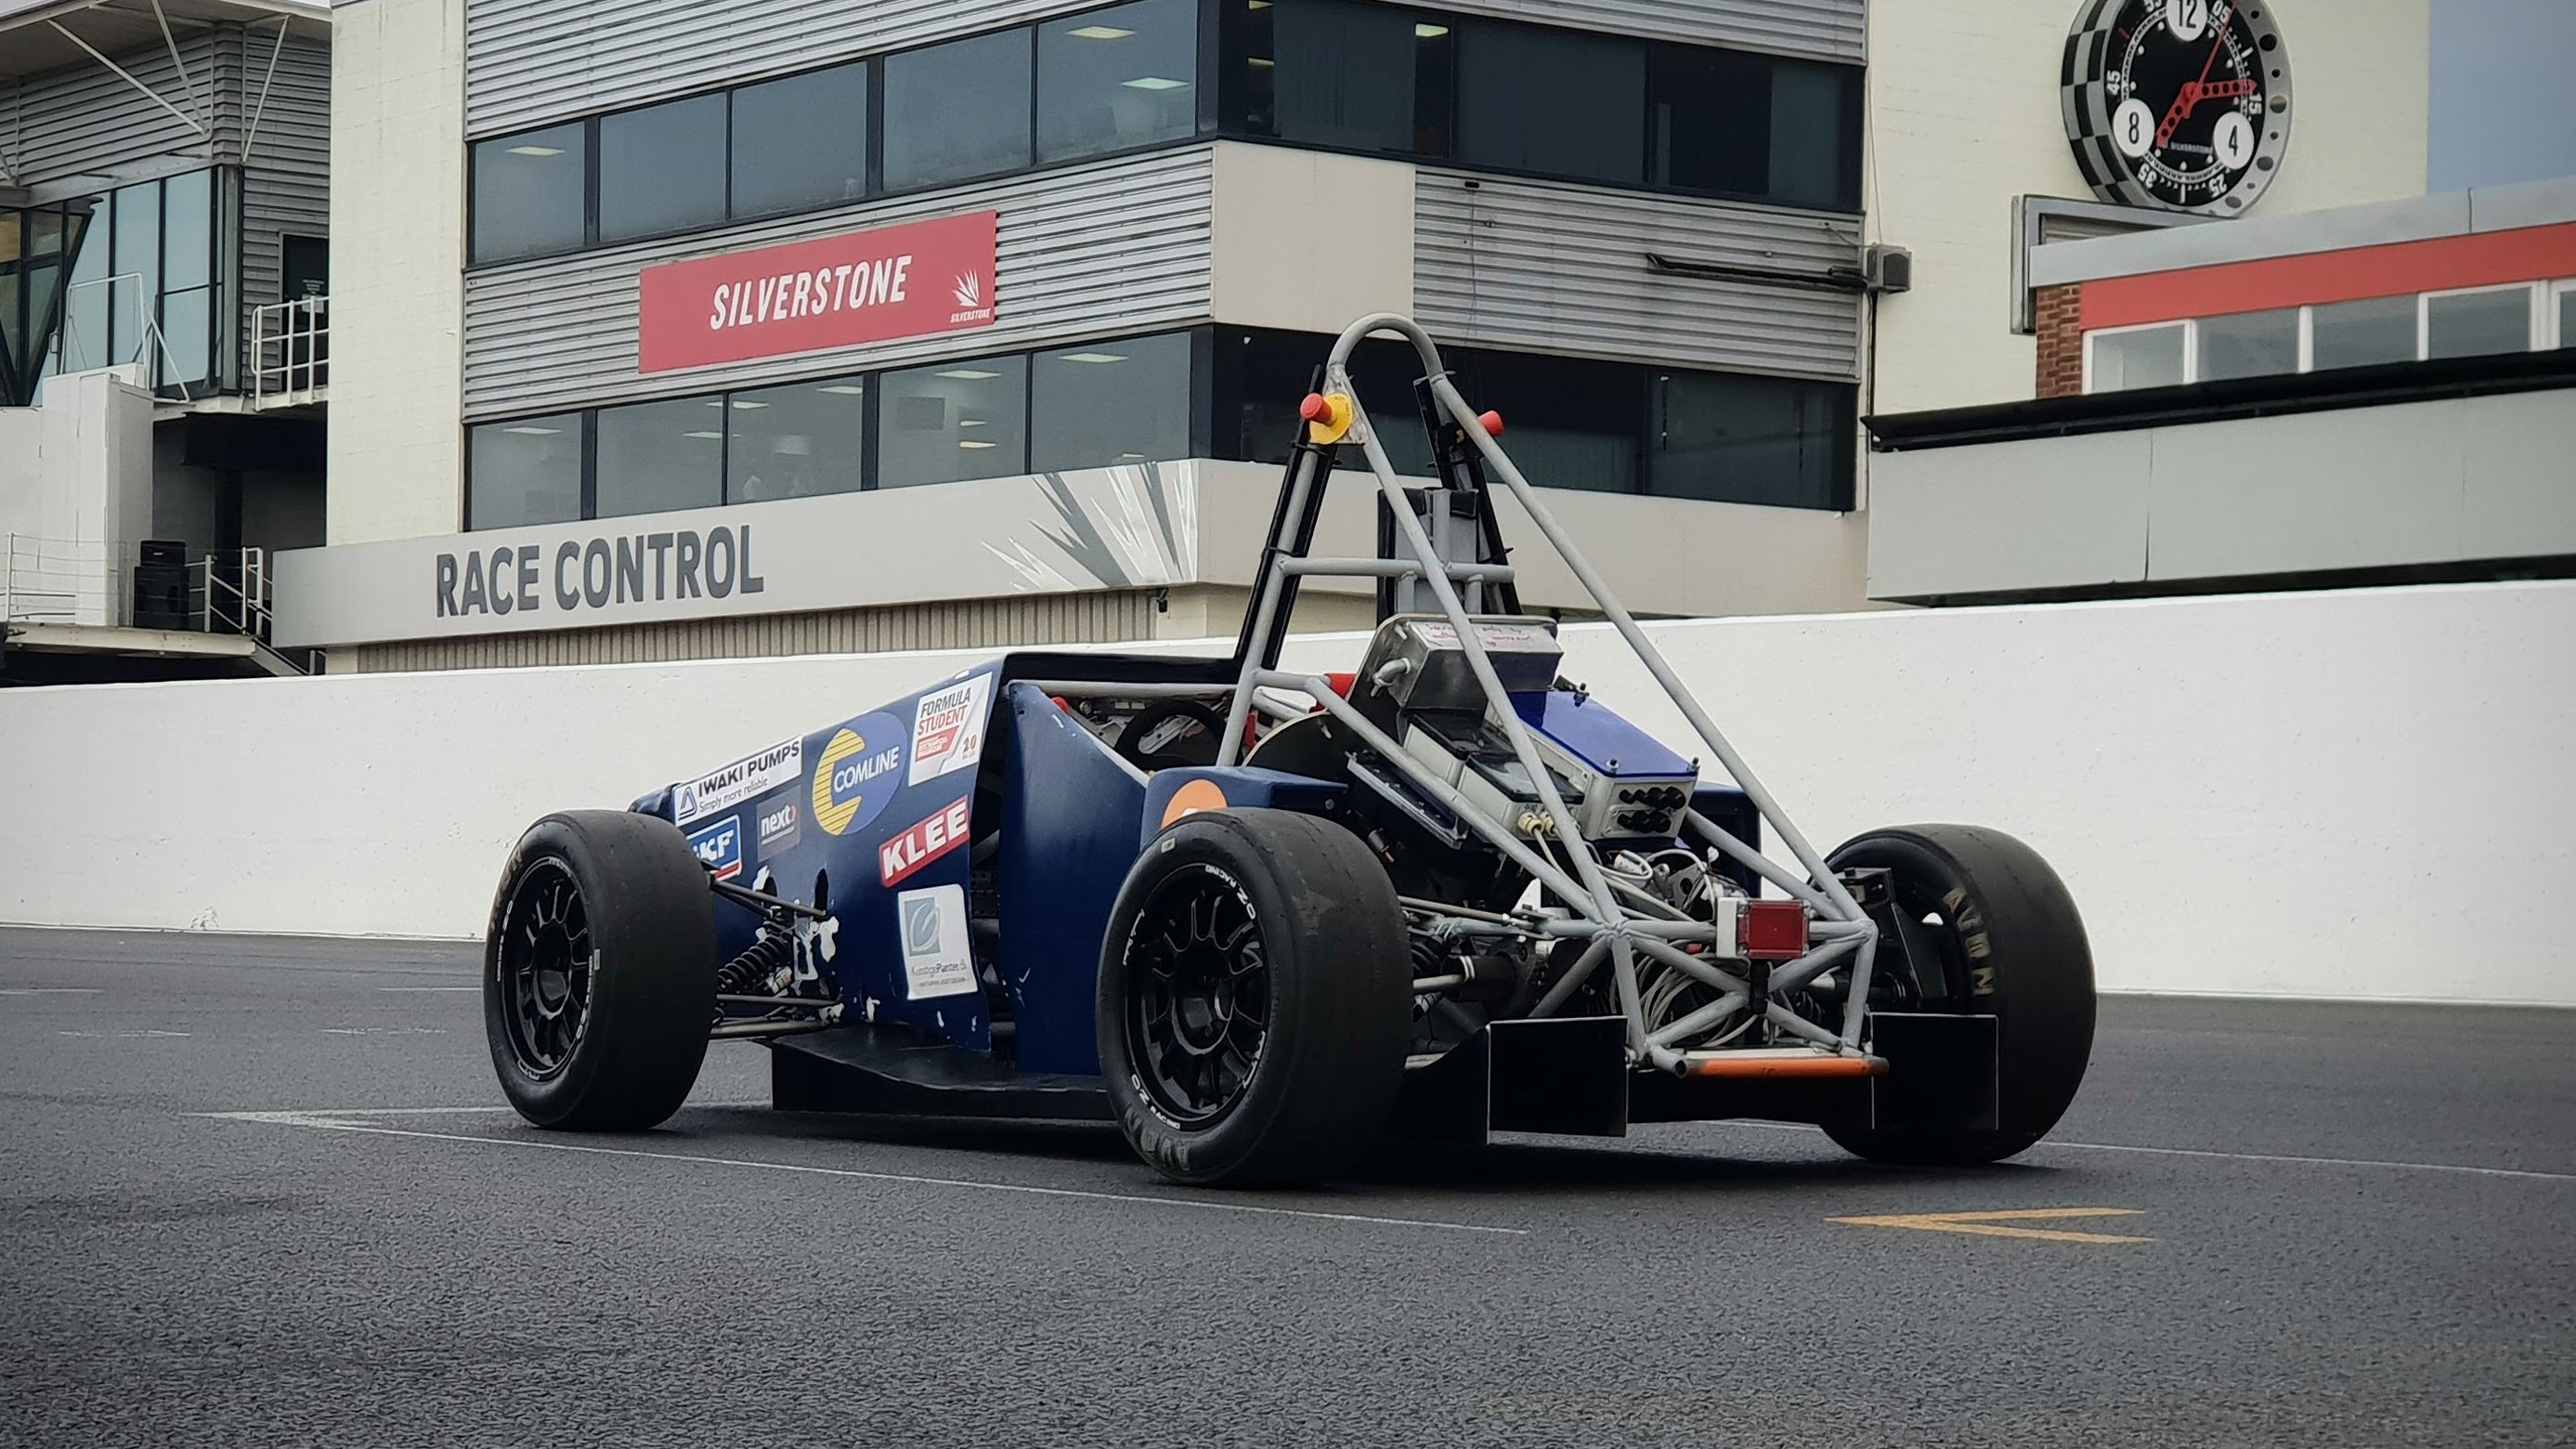
\includegraphics[width=0.8\textwidth]{figures/silverstone.jpg}
        \caption{Built car on Silverstone race circuit}
        \label{pic:silverstone}
\end{figure}


We have built an electric car from scratch based on a buggy frame, where all the pipes are welded together and all the components directly attached to it. Although in this solution, all the vibrations are transferred to the driver (reducing his comfort) it is a durable and light solution - the aspects which were the most important due to the racing character of the vehicle. 

Among many available options in our final setup we have used:
\begin{itemize}
    \item Two EMRAX228 motors where each of them is capable to work within continuous power of $28-42kW$\footnote{exact value depends on motor RPM}\cite{emrax_manual}
    \item Two emDrive500 controllers, implementing CANOpen protocol and being capable to make full usage of AM motors
    \item Arduino with CAN shields to act as intelligent sensors/controllers
    \item Two IWAKI direct drive pumps (RD-40E24-HN1V) for cooling purposes \todo{flow params?}
    % \begin{wrapfigure}
    %     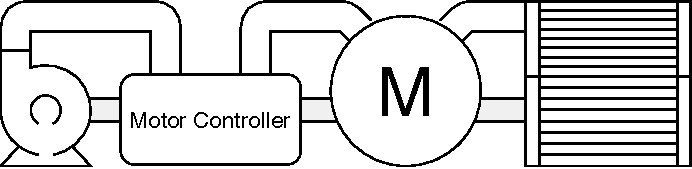
\includegraphics[width=0.33\textwidth]{figures/Pump.pdf}
    % \end{wrapfigure}
    \item National Instruments' cRIO-9033 as a main control unit
\end{itemize}
\newpage
This result in the system which in a simplified manner has been presented in figure \ref{fig:whole}.

\begin{figure}[h]
    \centering
    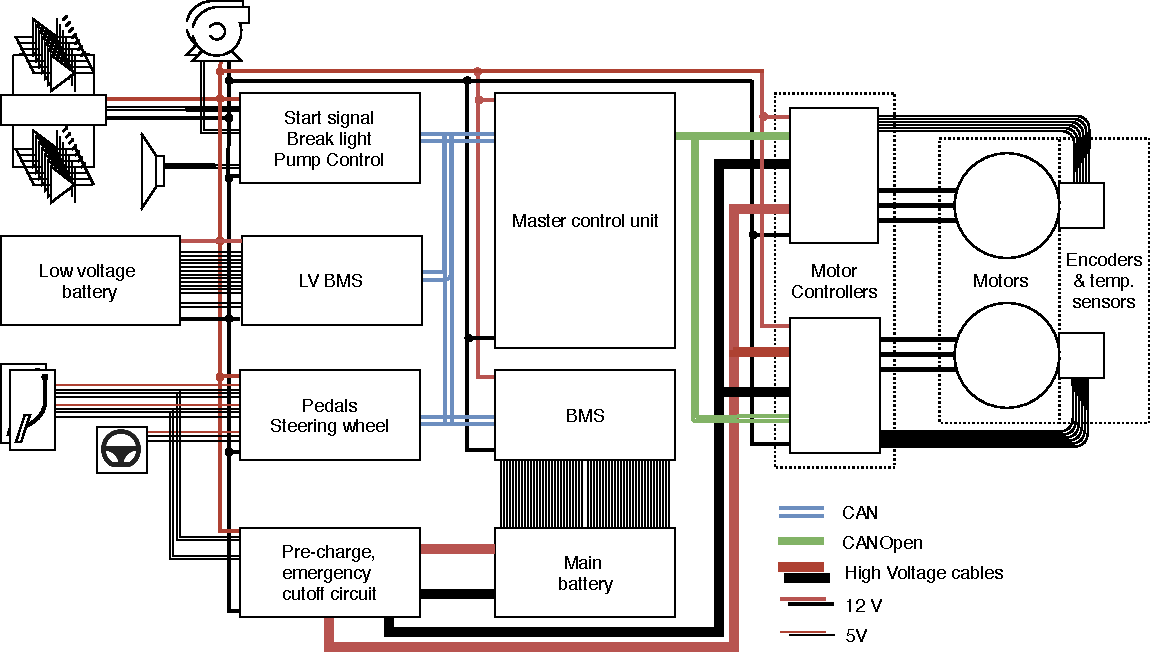
\includegraphics[width=\textwidth]{figures/Whole_with_details.pdf}
    \caption{Architecture overview}
    \label{fig:whole}
\end{figure}\todo{12V next to CAN + dashboard + LV to emc}

To start with in the left corner the breaking light has been shown, it operates on the 12V line and provides two levels of intensity (two sets of LEDs controlled independently). The control is based directly on CAN message send by pedals controller, providing additional functionality of lighting up if the connection is lost and blinking if pedals are sending the error messages.
To the right, we can see electrical buzzer (which is being used as ready to drive signal) and cooling pumps taking the same 12V and being controlled by a signal in between 0 and 5V. These all have been connected to the system by CAN adapter in the rear part of the car.

Other CAN module is a low voltage battery management system (LV BMS). It monitors each battery cell voltage and temperature, forwards this data to master control unit and cuts of low voltage battery out of circuit in case of any failures (voltage below operational or too high temperature).

Below the pedals/steering wheel intelligent sensor has been shown. It forwards the sensors values, provides a calibration interface and sends the errors due to under-travel, over-travel or sensors miss-match.

Another module is responsible for translating the CAN messages into indicator statuses on the dashboard and sensing the ignition buttons presses. 

Last but not least basic CAN device in the system is the BMS for the main battery, it monitors the cell state, provides load balancing and based on collected data deciding decides if the battery can be connected to the circuit.

The system which is completely independent to digital busses, emergency circuit, provides analogue circuits responsible for closing pre-charge relays and main contractors based on a variety of factors. The logic is based on pedals position (if accelerator and brake pedal are pressed simultaneously the main contractor is opened\footnote{Requirement by Formula Student}), LV BMS and main BMS.

If there are no safety issues AM system allows the voltage to flow into motor controllers. These devices are the only ones to communicate with the master control unit (MCU) by CANOpen bus. Beside MCU each controller is directly connected to the motor by three-phase cable\footnote{actually three separate cables to carry all the load}, to attached resolves and temperature sensors.

\section{Master control unit software implementation}
From the early beginning, I have been developing the code of master control unit using event-based programming paradigm. The reasoning of this is asynchronous, real-time nature of such unit.

Most simple classification of subsystems can be based on communication protocol being used. 

\subsection{Communication protocols}

\subsubsection{CAN integration}
To start with I had to implement a CAN library which would let me service messages from the code running on the real-time processor. I did it based on one of the provided examples, however, to meet my needs it required some ground modifications.

Especially functionality which has been missing is the ability to wait for a message with a certain id, one from an array of ids or just any message. 
\paragraph{Reading}

To achieve it, I have a functionality deployed on FPGA (Field Programmable Gate Array) which simply translates input/output messages into the arrays of 8x unsigned integers. Read messages are furthermore pushed into the FIFO register. In parallel, a consumer process is running which takes messages from the register set it as an output and raise an interrupt on the real-time processor to notify that data is ready to be read.

Upon initiation of the device, a programme is run on the real-time processor which besides the main process spawns an additional one in the background. This one furthermore is responsible for communication with the FPGA so whenever a message arrives it services interrupt by copying it and sends the acknowledge back to FPGA so next one can be transmitted. Meanwhile, CAN frame is stored in the table indexed by its ID and two notifications are sent (for the desired frame and for the arrival of any message)\footnote{Usage of LabVIEW synchronisation primitive "Queue".}% further described in \todo{queue description}}.

Now depending on a place in the code read function can be called in one of three ways:
\begin{description}[labelindent=1cm]
    \item[Read All] - function blocks the thread until notification arrives that any message has been received (or upon timeout) and returns it. Example of usage would be a logging purpose.
    \item[Read Some] - for given list of message IDs function behaves similarly to "Read All". However, notification is read and check if contains one of the listed IDs if not it starts again and return frame upon success (or error upon timeout). Example - Error handler.
    \item[Read ID] - waits for notification associated with the certain ID. Example - read pedal position.
    
%     Then look up table is check for the existence of a conditional variable for given id, it is created if does not exist, and updated with a new message. Additionally, a conditional variable containing the id of last received message id is updated.

% Based to this architecture I implemented functions which can wait for any message, one with a certain id or one from ids set.

\end{description}

\paragraph{Writing}
For sending a message it simply pushes data to FPGA and marks it as ready to send. FPGA is constantly checking the ready to send status and whenever it becomes true sends the data.

\vspace{5mm}
\noindent Thank this architecture CAN messaging part is easy to use, read and modify.

\subsubsection{CANOpen}
For the simplicity and maximum throughput although CANOpen is an abstraction layer over CAN bus an additional line has been used only for CANOpen communication. It has been used just to link two motor controllers and NI-9881 module (plugged into cRIO).

For the usage, CANOpen seemed like the best choice. It provides great flexibility in the way that all parameters can be accessed the way as they would be stored in memory registry without any pre-configuration. Furthermore, if setup correctly certain number of parameters can be accessed without any protocol overhead providing maximum bus throughput.

As previously mentioned in \ref{can_subprotocol} CANOpen abstraction consists of 6 complementary sub-protocols.
\begin{description}[labelindent=1cm]
    \item[NMT] Network management - Provides unified control over the devices state (Boot up, Pre-operational, Operational, Stopped)
    \item[SDO] Service Data Object - verbose protocol by default providing access to all the parameters of the device, it works based on two messages schema first describing which data should be sent next then in second sending actual data
    \item[PDO] Process Data Object - configurable sets of parameters to send/receive upon change or after SYNC message
    \item[SYNC]    Synchronisation Object - issue request of device status
    \item[TIME]    Time Stamp Object - is used to synchronise with device clock and it had no use in this project
    \item[EMCY] Emergency Object - asynchronously broadcast errors
\end{description}

As it meant to be I implemented one drive control based on NMT, SDO, PDO and SYNC protocols. Using NMT to control general state, SDO to control all the parameters before setting the device into operational mode and control device-specific states and PDO combined with SYNC messages to read device status and send control messages.

However, as it came to controlling two motors simultaneously conflicting messages ids in PDO and SYNC protocols needed to be changed. Although many tries it was not possible to change this values. Contacting the manufacturer drop the light on the case as they were aware that their devices malfunctions and were not able to provide any fix for the issue.

So for the two motor configuration, I had to implement a workaround by using slower and not providing all the functionality SDO protocol.
Usage of this protocol caused a drastic drop in channel throughput considering for instance reading of device status:
\begin{table}[H]
\centering
\begin{tabular}{|l|c|}
    \hline
    Data & Data size [byte] \\
    \hline
    Status word & 2 \\
    Controller Temperature & 1 \\
    Motor Temperature & 1 \\
    Error Code & 2  \\
    Error Register & 1 \\
    Torque Actual Value & 2  \\
    Velocity actual Value & 4  \\
    Electrical Angle & 2  \\
    Electric Power & 4 \\
    \hline
    \hfill Sum & 19 \\
    \hline
\end{tabular}
\caption{Motor controller status component sizing}
\end{table}

As each PDO message can contain up to 8 bytes aforementioned list of parameters would need to be divided into 3 CAN frames and as an result $46bits*3+19bytes+\epsilon = 290 bits +\epsilon$  \hspace{0.2cm}\footnote{\label{foot:eps}$\epsilon$ has been used to represent stuffed bits} needs to be send. On the other hand sending the same data with SDO protocol requires request-respond schema for each value so $46bits*18 + 19bytes + 9*4bytes + \epsilon = 1268 bits + \epsilon$ \hspace{0.2cm} \ref{foot:eps} needs to be send.

\begin{figure}[H]
    \centering
    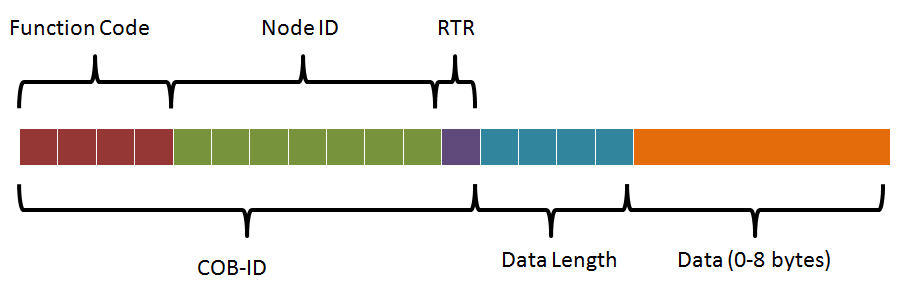
\includegraphics[width=0.8\textwidth]{figures/CANOpen_vs_CAN}
    \caption{CANOpen vs CAN}
    \label{fig:canopen_bitwise}
\end{figure}
    \todo{enrich it by missing fields}

Furthermore, also the target torque off motor controllers needs to be adjusted SDO messages. In this case, performance drawback is even more visible, if the PDO protocol could be used torque values could be sent together within one CAN frame ($46bits+4bytes=78 bits$), however, within SDO 4 CAN frames needs to be sent ($46bits*4+4bytes+4bytes*2=280bits$).

\subsection{Device operation states}

\begin{wrapfigure}{R}{0.43\textwidth}
    \vspace{-20pt}
    \centering
        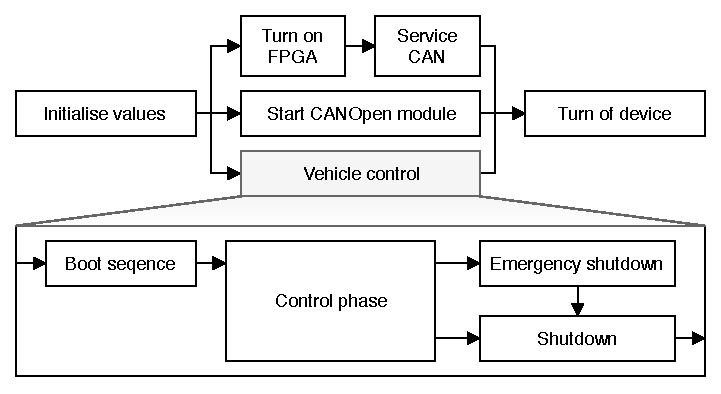
\includegraphics[width=0.4\textwidth]{figures/System_overview}
        \label{fig:sys_over}
        \caption{Control unit\newline states overview}
    \vspace{-20pt}
\end{wrapfigure}

The implemented control unit in practice consists of few nested state machines. The most general consist of just 3 states responsible for controller booting, operational and shutdown.
In booting state all initial values are set and internal modules like FPGA, CAN and CANOpen are being turned on in parallel to main threads. Whenever this phase is finished, an error logger is turn on and the car booting sequence begins.

To start with, the dashboard is updated with batteries charge status and systems waits for power up button to be pressed. Whenever driver would command turning of the vehicle button blinks and lights up by internal LED whenever BMS would response with ready to discharge message. Then the second button is required to be pressed in order to turn the traction system on (analogical interface to the first button). Whenever the traction system is first turned on, the controller sends a message to the audio-visual system so the car plays loud sound alerting the surrounding to take cautions as systems are charge and it is ready to drive.

In the operational state, many control loops run in parallel to cover desired vehicle functionality.
\begin{itemize}
    \item Pedals status is read, updates local pedal status and issue notification that motor controllers should be updated with new values. 
    \item Upon notification new target torques values are calculated and send to motor controllers.
    \item Running watchdog, if no pedals update was notified within 500ms set target torques to zero (an emergency mechanism to slow the motors in case of any temporary fail of pedals sensor).
    \item Set pumps to full power for 3s to initiate rotation, then control it accordingly to further mentioned method.\ref{pump_control}
    \item Communicate with BMS to keep it in an operational state.
    \item Read and act upon BMS and low voltage BMS state.
    \item Log all the information.
\end{itemize}


\section{Pedals sensor}
A System to measure pedals and steering wheel position is based on Arduino evaluation board. Which is a simple evaluation setup build upon Atmel ATmega8 with $16MHz$ oscillator.

Now considering the sampling rate of this sub-module it has been programmed to use prescaler for A/D converter with a value of 128. Referring to datasheet basic conversion takes 13 clock cycles so we should except sampling rate of about $16MHz/128/13 = 9615Hz = 104µs$ \cite{Atmega8}.

However, in an electric car, there is a considerable electromagnetic noise which needs to be addressed. To reduce the impact of noise which was significant in the first approach, the code was modified to calculate an average of 10 successive samples efficiently reducing the rate to $1,04ms$.

Considering the fact that ATmega8 consist of just one analogue-decimal converter with multiplexed input the measurement takes approximately $1,04ms * number of sensors$ \cite{Atmega8}.
To satisfy the safety requirements we needed to use two offset sensors for each pedal (accelerator, brake) and one for the steering wheel. In consequence each measurement takes at least $1,04ms * 5 = 5,2ms$.

This system sense all the information which is:
\begin{itemize}
    \item pedals position
    \item steering wheel position
    \item pedals sensors position miss-match
    \item pedals, steering wheel over-travel, under-travel and connection loss errors
\end{itemize}

After the measurement, the information is sent through CAN bus with a baud rate of 500kbit/s (used CAN module was not capable to work with higher baud rates). Pedals position although being read on 10 bits is averaged and only 8 significant bits are sent. We assumed that 256 quantization steps are sufficient in this case. It allowed us to shorten CAN frame to consist of only 4 bytes of data.
Now considering timing, the CAN frame (\ref{fig:CAN_FRAME}) consists of at least 44 basic bits plus 4 bytes of data in our case. The total time of sending/receiving would be therefore $\frac{76}{500kbit/s} = 152us$.

\begin{figure}[H]
    \centering
    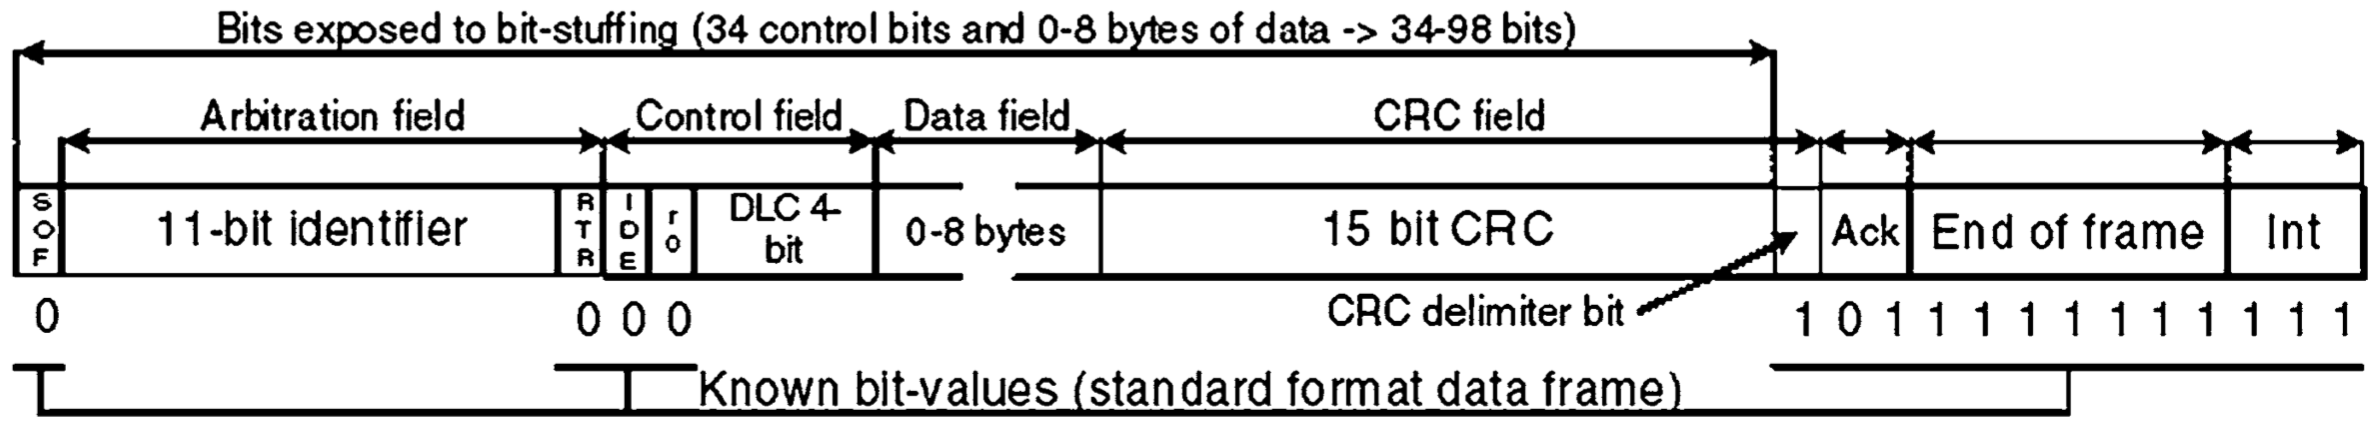
\includegraphics[width=0.9\textwidth]{figures/CAN_FRAME.png}
    \caption{CAN frame structure \cite{CAN_stuffing}}
    \label{fig:CAN_FRAME}
\end{figure}

Assuming no further improvements we should expect the pedals sub-systems is capable of sending the pedals, steering wheel position in a time interval of about $5,2ms$\label{pedal_ideal_time} in normal operation.
Additionally, if any of the above-mentioned errors occurred the second CAN frame is sent containing two bytes with bitwise encoded errors extending the expected interval into $~5,3ms$.

\section{Pump control}\label{pump_control}
In our car, we have used IWAKI RD-40E24-HN1V pumps, which can be controlled by a signal from $0-5V$. Since used Arduino has no dedicated analogue input we made one by using the PWM signal with a low-pass filter.% (direct control by PWM signal was strongly disapproved by the pump manufacturer \todo{cite pump manual}). <= I was told that by mech guys but there is no single word in manual
The subsystem acts simply by controlling pulse width based on the value received by CAN message from the master control unit. It also provides basic emergency behaviour in the manner that if no message was sensed over one second the pumps are turned on to work with full power.

When it comes to choosing the right pump power the simplest approach would be to simply relay on feedback loop (fig. \ref{pump_feedback}). Which, assuming sufficient cooling pump performance, is capable of keeping the motors within preset operational temperature scale in static conditions. However, considering sudden acceleration this system respond could be too slow letting the temperature rise above permit limits.
To reduce response time I have used additional feed-forward control (\ref{pump_forward}) taking as an input an accelerator position, which should be proportional to used motor power (heat dispatch).

\begin{figure}[H]
    \def\visc{0.8}
    \centering
    \subbottom[Pump control in feedback loop]{
        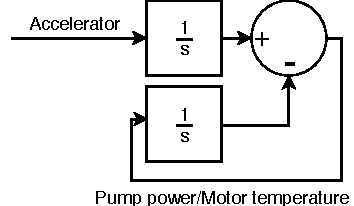
\includegraphics[scale=\visc]{figures/Pump_feedback}
        \label{pump_feedback}
    }
    ~
    \subbottom[Pump control with feedback loop and feed forward patch]{
        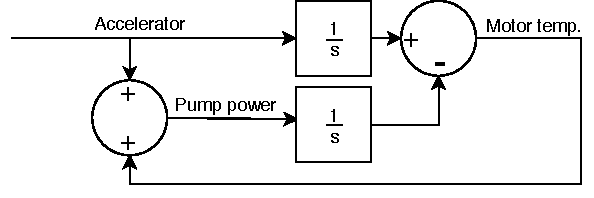
\includegraphics[scale=\visc]{figures/Pump_forward}
        \label{pump_forward}
    }
    \caption{Pump control}
    \label{vi:set_get_nodeid}
    \medskip
    \small
    \textit{The parameters coefficients has been omitted for simplicity}
\end{figure}

The pump power, therefore, is calculated accordingly to the following equation:
\begin{equation}\label{pump_eq}
    \tau_{left,right} = \begin{cases}
        P_{pump} = 50\% & \text{se $T<T_{min}$}\\
        P_{pump} = 50\%+coerce(norm(T) + D)*50\% & \text{se $T \in <T_{min},T{max}>$}\\
        P_{pump} = 100\% & \text{se $T>T{max}$}
    \end{cases}
\end{equation}
Where:
\begin{description}
    \item[$P_{pump}$] pump power in percentage
    \item[T] higher on of two motor temperatures
    \item[\textbf{$T_{min}$, $T{max}$}] operational temperature limits in this case equal to $40^\circ C$ and $60^\circ C$
    \item[coerce()] returns value limited to $<0,1>$
    \item[norm(T)] $=coerce(\frac{T - T_{min}}{T_{max}-T_{min}})$ 
    \item[D] acceleration pedal displacement in percentage
\end{description}

\section{Implementation of electrical differential based on steering angle}\label{diff_meth}
In my implementation I have enriched calculations explained in \ref{diff_calc}. Starting with the steering wheel, the sensor output is normalised to the measured minimum and maximum steering wheel angles ($\pm123\deg$) so the meaningful value can be shown in remote control panel as well as saved in logs. 
Then since it is linearly proportional it is simply converted to steering angle ($\pm35\deg$). To prevent any miss usage all the values are coerced on the go to be within the ranges.

Having commanded output power (in percentage) basic differential functionality could be obtained just by multiplying it with a maximum allowed/available torque and proportion on per wheel base. However, it would start failing for power close to $100\% $, although total torque will remain under the limit, the outer wheel can go above the limit by up to ($20\% $).
This situation would be especially dangerous if the maximum torque per wheel base would start to saturate. In this case, the differential would gradually stop to function effectively by pushing the car out of the desired curve.
To avoid this miss-behaviour I added the code to check if after previous calculation any of the wheels is about to be set to more than maximum torque and scale both of them accordingly.
\begin{equation}\label{diff_saf}
    \tau_{left,right} = \begin{cases}
        \tau_{left,right} = P * \gamma_{left,right} * \tau_{max} & \text{se $m(P,\gamma_{left,right}) \leq 1$}\\
        \tau_{left,right} = P * \gamma_{left,right} * \tau_{max} / m(P,\gamma_{left,right}) & \text{se $m(P,\gamma_{left,right}) > 1$}\\
    \end{cases}
\end{equation}
Where:
\begin{description}
    \item[P] desired output power ($0-100\%$)
    \item[$\tau_{max}$] maximum torque per wheel
    \item[$\tau$] wheel torque
    \item[$\gamma$] differential disproportion of wheel ($\gamma_{left}+\gamma_{right}=200\%$)
    \item[$m(P,\gamma{left,right})$] $= P * max(\gamma_{left},\gamma_{right})$
\end{description}

\section{Regenerative braking}
As mentioned in theory chapter (\ref{regenerative_theory_section}) the regenerative braking cannot be used in low speeds. Normally this problem would be solved by varying the braking force between regenerative and friction breaks. However, the car design did not take into the account the possibility to electrically control the friction breaks. So I implemented an alternative solution taking into account this technical obstacle and comfort of the driver.
Considering regenerative braking as negative torque system which I have implemented can be expressed by equation \ref{reg_break_eq}.


\begin{equation*}
    \tau = \begin{cases}
        D & \text{se $V_{avg} \leq 10km/h$}\\
        (V_{norm,10-20} * 15\% + 100\%) * D - V_{norm,10-20} * 15\% & \text{se $V_{avg} \in (10km/h,20km/h>$}\\
        115\% * D - 15\% & \text{se $V_{avg} > 20km/h$}\\
    \end{cases}
    \label{reg_break_eq}
\end{equation*}
Where:
\begin{description}
    \item[$V_{avg}$] average velocity of the wheels 
    \item[$V_{norm,10-20}$] $V_{avg}$ normalised in range from 10 to 20 ($V_{norm,10-20}=(V_{avg}-10)/10$)
    \item[D] acceleration pedal displacement in percentage
    \item[$tau$] percentage of used torque (in reference to maximum value)
\end{description}

It follows the simple idea to use a variable portion of pedal displacement for regenerative braking based on speed.
When the user presses the acceleration pedal in a stationary vehicle the whole available scale is used to control torque giving an expected instant response. After reaching $10km/h$ the pedal displacement used for regenerative braking increases gradually to reach $15\%$ while travelling with speed equal to or higher than $20km/h$.

What else is worth to mention is that as a result for the pedal displacement from $0-15\%$ we should expect the car to act as it would be controlled in speed mode.\label{speed_mode} The characteristic would be firstly saturated by low torque however within enough power to make the car accelerate we should be able to observe a linear correlation between pedal displacement and speed.

To summarise the expected idealised correlation between torque, pedal displacement and speed has been shown in figure \ref{fig:regen_ideal}.

\begin{figure}[H]
    \centering
        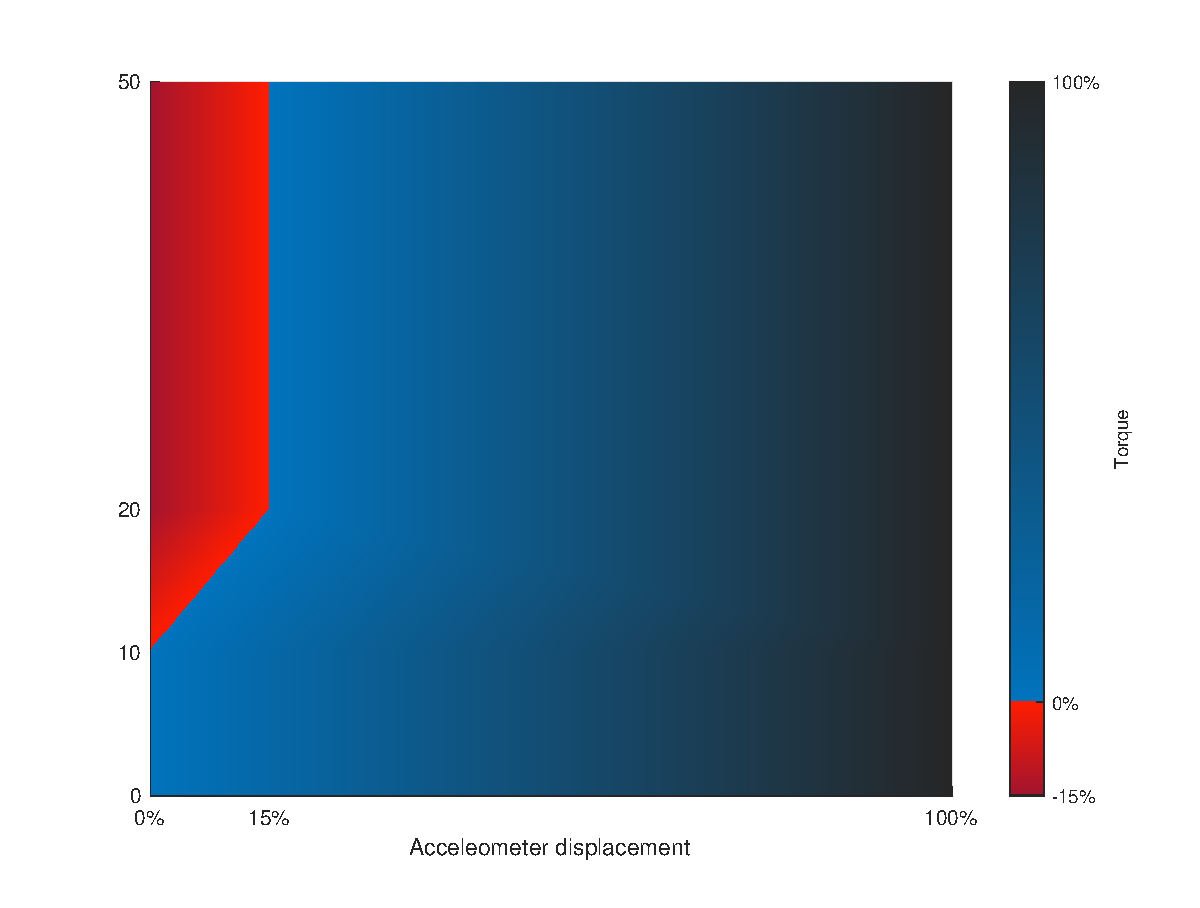
\includegraphics[height=5.8cm]{figures/regen_ideal}
        \caption{Regenerative braking / torque control}
        \label{fig:regen_ideal}
\end{figure}